\section{Honeypots in the Cloud}

\begin{frame}{Cloud Providers}
    \begin{columns}
        % Column 1
        \begin{column}{0.25\textwidth}
            \begin{figure}
                \centering
                
\includegraphics[width=\columnwidth]{img/heicloud_logo.png}
            \end{figure}
        \end{column}
        % Column 2
        \begin{column}{.02\textwidth}
            \rule{.1mm}{0.7\textheight}
        \end{column}
        % Column 3
        \begin{column}{0.25\textwidth}
            \begin{figure}
                \centering
                
\includegraphics[width=0.5\columnwidth]{img/aws_logo.png}
            \end{figure}
        \end{column}
        % Column 4  
        \begin{column}{0.25\textwidth}
            \begin{figure}
                \centering
                
\includegraphics[width=\columnwidth]{img/gcp_logo.png}
            \end{figure}
        \end{column}
        % Column 5
        \begin{column}{0.25\textwidth}
            \begin{figure}
                \centering
                
\includegraphics[width=0.5\columnwidth]{img/azure_logo.png}
            \end{figure}
        \end{column}
    \end{columns}
\end{frame}

\begin{frame}{Introduction}
    \begin{block}{\citet{Spitzner2003}}
        Any activity sent their way (to a honeypot) is suspect by nature.
    \end{block}
\end{frame}

\begin{frame}{Introduction}
    Trying to answer the questions:
    \begin{itemize}
        \item Do honeypots help to detect bot activities?
        \item What are buzzing attacks nowadays?
        \item Is heiCLOUD a preferred target?
    \end{itemize}
\end{frame}

\begin{frame}{Concept}
    \begin{columns}
        % Column 1
        \begin{column}{0.5\textwidth}
            \begin{itemize}
                \item Using latest T-Pot version
                \item Allow all incoming TCP and UDP connections
                \item Capturing attacks over 3 weeks
            \end{itemize}
        \end{column}
        % Column 2
        \begin{column}{.02\textwidth}
            \rule{.1mm}{0.7\textheight}
        \end{column}
        % Column 3
        \begin{column}{0.5\textwidth}
            \begin{figure}
                \centering
                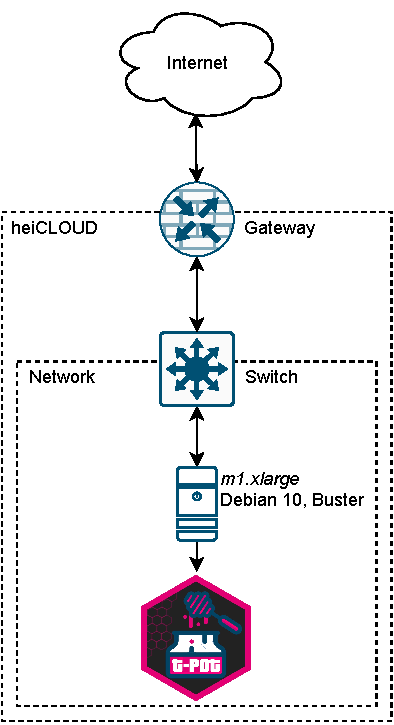
\includegraphics[width=0.7\columnwidth]{img/tpot-concept.pdf}
                \caption{Concept to gather attacks}
            \end{figure}
        \end{column}
    \end{columns}
\end{frame}

\begin{frame}{Results}
    \begin{figure}
        \centering
        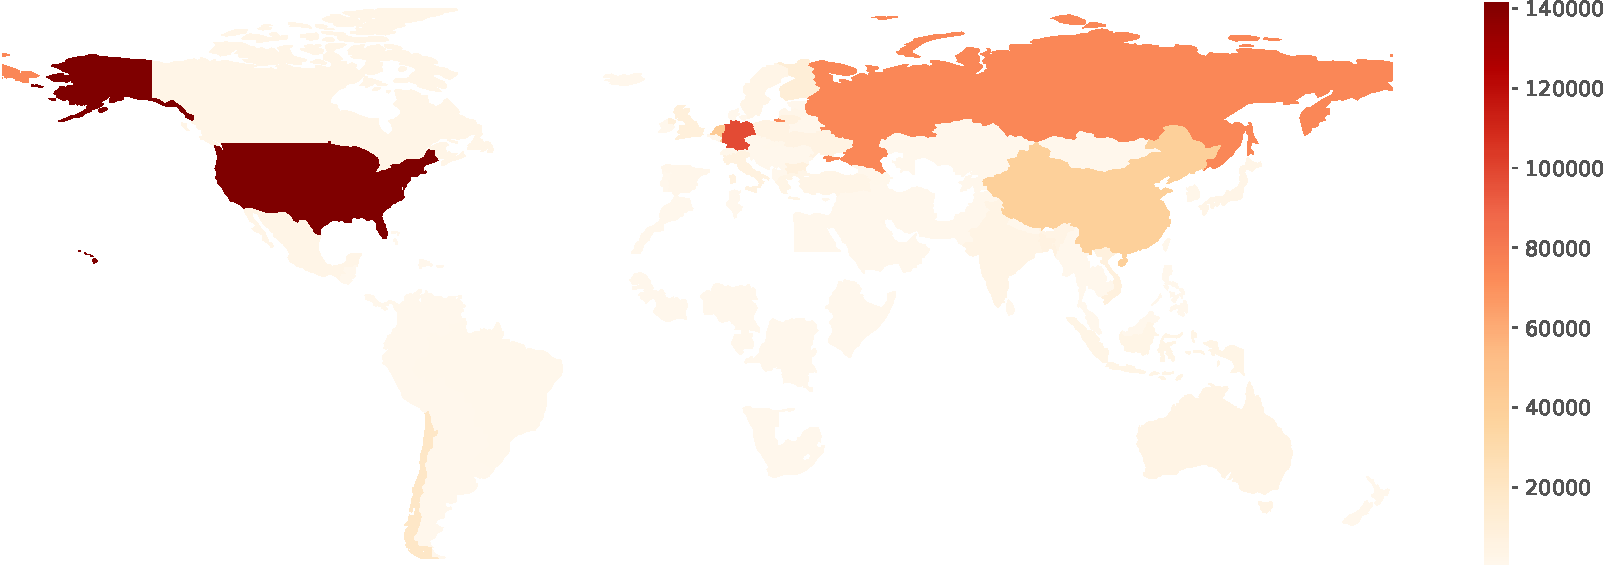
\includegraphics[width=\columnwidth]{img/tpot-overview-map.pdf}
        \caption[Attack distribution of T-Pot]{
            Attack distribution of T-Pot.
        }
        \label{fig:attack-distribution}
    \end{figure}
\end{frame}

\begin{frame}{Results}
    \begin{columns}
        % Column 1
        \begin{column}{0.4\textwidth}
            {\footnotesize
            \begin{itemize}
                \item Many RDP and VoIP alerts
                \item Focus on outdated Windows server
            \end{itemize}
            }
        \end{column}
        % Column 2
        \begin{column}{0.6\textwidth}
            \begin{figure}
                \centering
                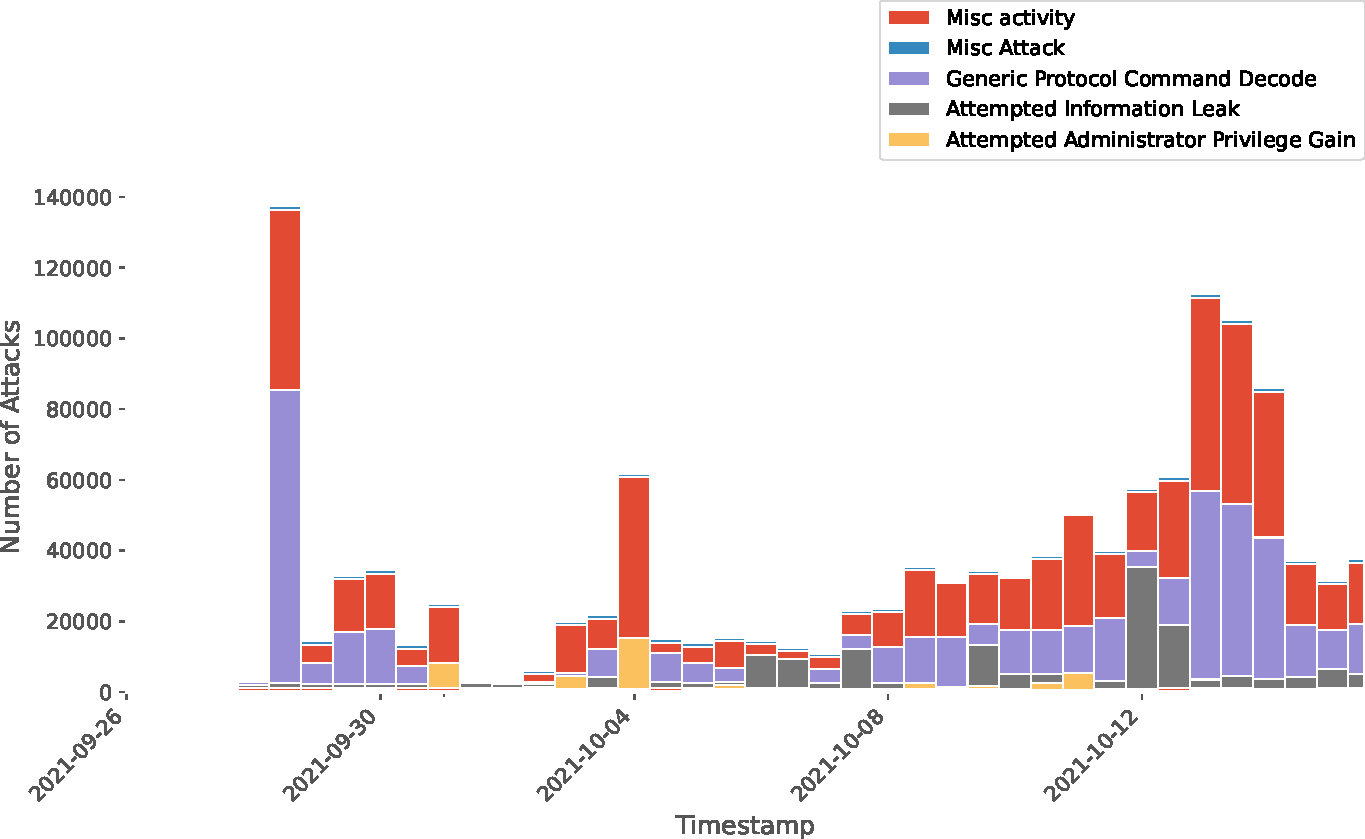
\includegraphics[width=\columnwidth]{img/tpot-suricata-alerts.pdf}
                \caption[Suricata results of T-Pot]{
                    Suricata results of T-Pot.
                }
                \label{fig:suricata-results}
            \end{figure}
        \end{column}
    \end{columns}
\end{frame}

\begin{frame}{Results}
    \begin{figure}
        \centering
        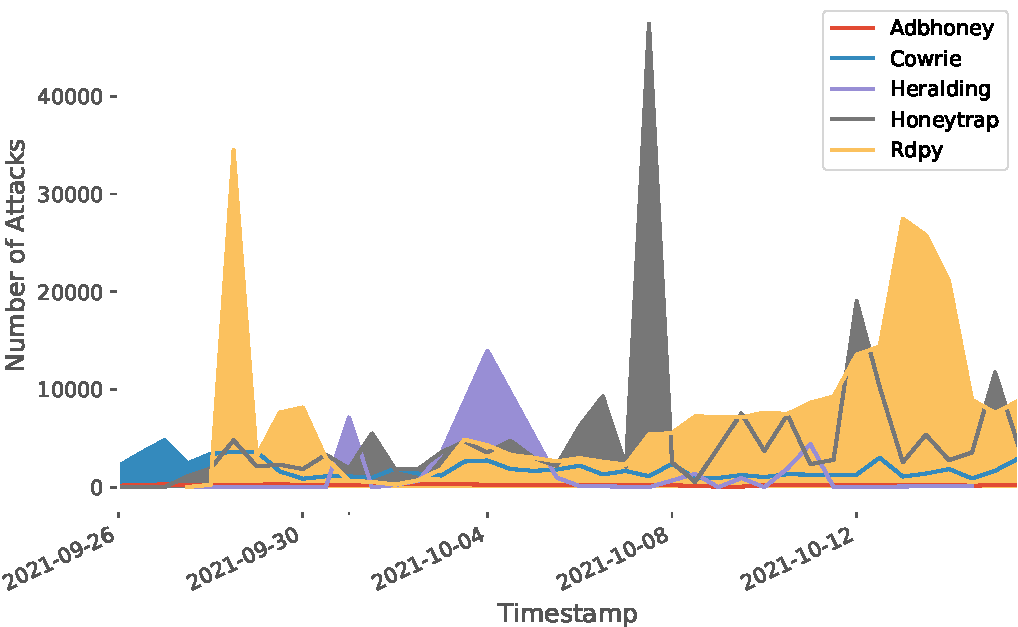
\includegraphics[width=\textwidth]{img/tpot-attacks-histogram.pdf}
        \caption[Attack histogram of T-Pot]{
            Attack histogram of T-Pot.
        }
        \label{tpot-overview-histogram}
    \end{figure}
\end{frame}

\begin{frame}{Results}
    \begin{figure}
        \centering
        \begin{subfigure}[b]{0.49\columnwidth}
            \centering
            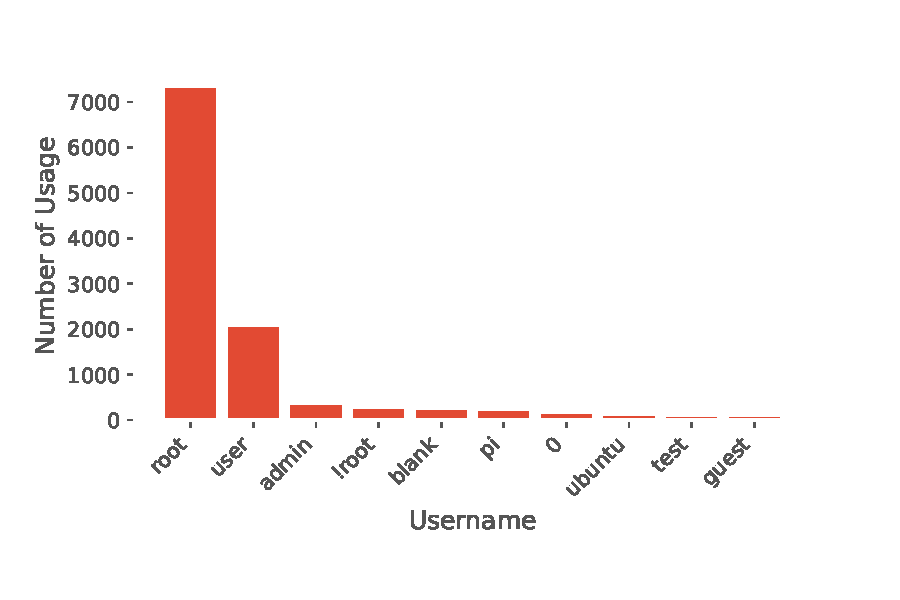
\includegraphics[width=\columnwidth]{img/tpot-cowrie-username.pdf}
            \caption{Cowrie username credentials}
            \label{fig:tpot-cowrie-username}
        \end{subfigure}
        \hfill
        \begin{subfigure}[b]{0.49\columnwidth}
            \centering
            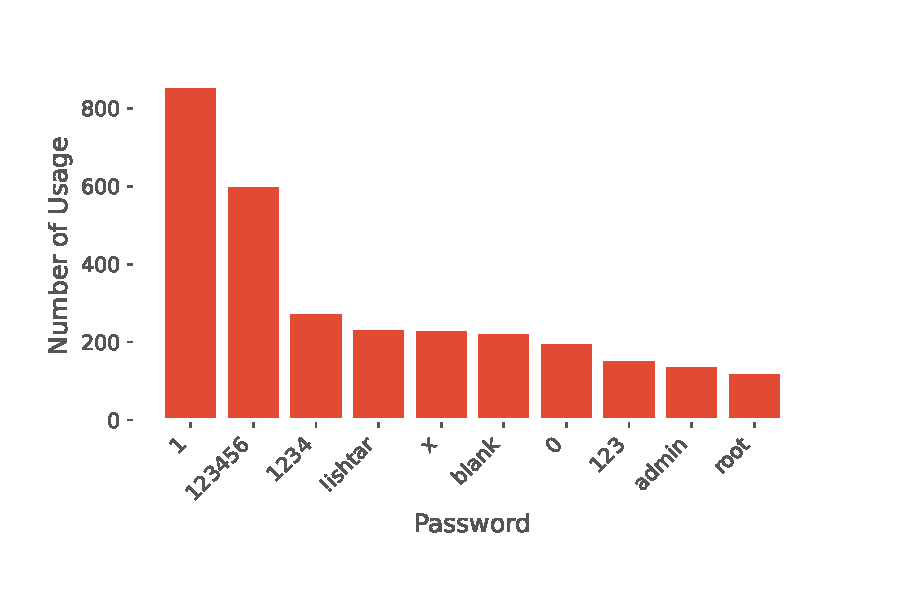
\includegraphics[width=\columnwidth]{img/tpot-cowrie-password.pdf}
            \caption{Cowrie password credentials}
            \label{fig:tpot-cowrie-password}
        \end{subfigure}
        \caption[Cowrie top 10 credentials on T-Pot]{
            Cowrie top 10 credentials used on T-Pot.
        }
        \label{fig:cowrie-credentials}
    \end{figure}
\end{frame}

\begin{frame}{Summary}
    \begin{itemize}
        \item Interesting to mention:
        \begin{itemize}
            \item Cryptocurrency attacks getting more popular
            \item Increase in RDP and VoIP attacks
            \item Quick adaption of new attacks (e.g. Apache 2.49.0 CVE)
        \end{itemize}
        \item Do honeypots help to detect bot activities?
        \begin{itemize}
            \item Yes
        \end{itemize}
        \item Is heiCLOUD a preferred target?
        \begin{itemize}
            \item Can not be confirmed
        \end{itemize}
    \end{itemize}
\end{frame}
